\documentclass[12pt, a4paper, twoside, openright]{Thesis} % Paper size, default font size and one-sided paper
\usepackage[utf8]{inputenc}
\usepackage{wrapfig}
\usepackage{lscape}
\usepackage{rotating}
\usepackage{graphicx}
\usepackage{caption}
\usepackage{amsmath, nccmath}
\usepackage{comment}
\usepackage{afterpage}
\usepackage{multirow}
\usepackage{multicol}
\usepackage{cleveref}
\usepackage{rotating}
% \usepackage[font=small]{caption}
% \captionsetup{compatibility=false}
% \usepackage{subcaption}
% \usepackage{subfig}
\usepackage{makecell}
\usepackage{booktabs}
\usepackage{multirow}
\usepackage{lscape}
\usepackage{longtable}
\usepackage{placeins}
\usepackage{adjustbox}
\usepackage{arydshln} % dashed midline
\usepackage{ragged2e}
\usepackage{lipsum}
\usepackage{mathtools} % To use box inside an aligned environment
\usepackage{enumitem} % for roman letter lists
\usepackage{listings}
\usepackage{algorithm}
\usepackage{algorithmic}
\usepackage{tabularx}
\usepackage{booktabs}
\usepackage{xcolor}
\usepackage{amsmath}

\definecolor{codegreen}{rgb}{0,0.6,0}
\definecolor{codegray}{rgb}{0.5,0.5,0.5}
\definecolor{codepurple}{rgb}{0.58,0,0.82}
\definecolor{backcolour}{rgb}{0.95,0.95,0.92}

\lstdefinestyle{mystyle}{
    backgroundcolor=\color{backcolour},   
    commentstyle=\color{codegreen},
    keywordstyle=\color{magenta},
    numberstyle=\tiny\color{codegray},
    stringstyle=\color{codepurple},
    basicstyle=\ttfamily\footnotesize,
    breakatwhitespace=false,         
    breaklines=true,                 
    captionpos=b,                    
    keepspaces=true,                 
    numbers=left,                    
    numbersep=5pt,                  
    showspaces=false,                
    showstringspaces=false,
    showtabs=false,                  
    tabsize=2
}

\lstset{style=mystyle}


% \usepackage{subfig}
\newcommand\myemptypage{
    \null
    \thispagestyle{empty}
    \addtocounter{page}{-1}
    \newpage
    }
%\usepackage[width=14cm, left=3cm]{geometry}

% prints author names as small caps


%\usepackage{subcaption} %incompatible with subfig
\graphicspath{{Pictures/}} % Specifies the directory where pictures are stored
% \usepackage[authoryear]{natbib}
% \usepackage[square, numbers]{natbib} % Use the natbib reference package - read up on this to edit the reference style; if you want text (e.g. Smith et al., 2012) for the in-text references (instead of numbers), remove 'numbers' v
% \bibliographystyle{abbrvnat}
% \setcitestyle{authoryear,open={((},close={))}}
\usepackage[english]{babel}
\usepackage[square,numbers]{natbib}
\bibliographystyle{abbrvnat}

\hypersetup{urlcolor=blue, colorlinks=true} % Colors hyperlinks in blue - change to black if annoyingv`	
\title{\ttitle} % Defines the thesis title - don't touch this




%%%% New added


\usepackage{tikz}
\usetikzlibrary{shapes.geometric, arrows}

% Defining Tickz Style
\tikzstyle{startstop} = [rectangle, rounded corners, minimum width=3cm, minimum height=1cm, text centered, text width = 10cm, draw=black, fill=white]

% \tikzstyle{startstop1} = [rectangle, rounded corners, minimum width=3cm, minimum height=1cm, text centered, draw=black, fill=white, text width = 10cm]

% \tikzstyle{io} = [trapezium, trapezium left angle=70, trapezium right angle=110, minimum width=3cm, minimum height=1cm, text centered, text width = 4.5cm, draw=black, fill=blue!30]

\tikzstyle{process} = [rectangle, minimum width=3cm, minimum height=1cm, text centered, text width = 6cm, draw=black, fill=white, text width = 10cm]

% \tikzstyle{decision} = [diamond, minimum width=3cm, minimum height=1cm, text centered, draw=black, fill=green!30]

\tikzstyle{arrow} = [ultra thick,->,>=stealth, line width=0.7mm]







\usepackage[T1]{fontenc}

\begin{document}
% \makeatletter
% \renewcommand*{\NAT@nmfmt}[1]{\textsc{#1}}
% \makeatother

% prints author names as small caps
% it is sometimes necessary in user documents to have access to such package-internal macros, and so the commands \makeatletter and \makeatother change the catcode 


\frontmatter % Use roman page numbering style (i, ii, iii, iv...) for the pre-content pages

\setstretch{1.6} % Line spacing of 1.6 (double line spacing)

% Define the page headers using the FancyHdr package and set up for one-sided printing
\fancyhead{} % Clears all page headers and footers
\rhead{\thepage} % Sets the right side header to show the page number
\lhead{} % Clears the left side page header

\pagestyle{fancy} % Finally, use the "fancy" page style to implement the FancyHdr headers

\newcommand{\HRule}{\rule{\linewidth}{0.5mm}} % New command to make the lines in the title page

% PDF meta-data
\hypersetup{pdftitle={\ttitle}}
\hypersetup{pdfsubject=\subjectname}
\hypersetup{pdfauthor=\authornames}
\hypersetup{pdfkeywords=\keywordnames}




% --------------------------------------------------





%----------------------------------------------------------------------------------------
%	TITLE PAGE
%----------------------------------------------------------------------------------------
\begin{comment}
\begin{titlepage}
\begin{center}

\HRule \\[0.4cm] % Horizontal line
{\huge \bfseries \ttitle}\\[0.4cm] % Thesis title
\HRule \\[1.5cm] % Horizontal line
 
\large \textit{A thesis submitted in fulfillment of the requirements\\ for the degree of \degreename}\\[0.3cm] % University requirement text
\textit{by}\\[0.4cm]

%\href{http://home.iitk.ac.in/~saiwal}{\authornames}

\vfill
\graphicspath{ {./Figures/} }
\begin{figure}[hb]
  \centering
  \includegraphics[width=0.4\linewidth]{Images/redlogo.png}
\end{figure}

\DEPTNAME\\ % Research group name and department name
\textsc{ \UNIVNAME}\\[1.5cm] % University name
\large \today\\[2cm] % Date


\end{center}

\end{titlepage}
\end{comment}
%\begin{document}
%\begin{titlepage}


%\include{title1}
%\end{titlepage}
%\myemptypage
%\afterpage{\null\newpage}
%\include{blank_page_1}
%\newpage
%\newpage
%\newgeometry{centering,top = 2.54cm,bottom = 2.54cm,left = 2.54cm, right = 2.54cm, includeheadfoot}

\pagenumbering{gobble}% Remove page numbers (and reset to 1)
\thispagestyle{empty}
\singlespacing
\begin{titlepage}
%\setlength{\voffset}{-0.1in}
%\setlength{\headsep}{5pt}
%\setlength{\textheight}{650pt}
%titlepage
%\thispagestyle{empty}
\begin{center}
%\begin{minipage}{0.75\linewidth}
    \centering
     
%=====================================================%
%---------------THESIS TITLE--------------------------%
%=====================================================%    
\definecolor{blue}{rgb}{0,0,1} % before using a colour one has to define it like this, here you have given color with rgb as 0,0,1 as blue
      
  {{\Large \textbf{Design and Implementation of a Quantized CNN Inference Engine  on FPGA
}\par}}
    \vspace{1cm}% FOR CREATING DESIRED SPACE BETWEEN THE LINES
     
%=====================================================%
%---------------Partial Fulfillment---------------------%
%=====================================================%
    \vspace{1cm}
    {Dissertation submitted in partial fulfilment of the requirements \\ for the award of 
    \par}
    \vspace{0.1cm}
    {
    \textbf{\large Dual Degree(B.Tech and M.Tech)} \par}
    \vspace{0.3cm}

%=====================================================%
%---------------AUTHOR'S NAME-------------------------%
%=====================================================%

    {\large by\par}
    \vspace{0.1cm}
    {\large \textbf{\textcolor{blue}{Vennapusa Indrahas Reddy}}\par} 
    (Roll No. 19D070067)
%    {\Large \textbf{(2013MEZ8469)}\par}
    \vspace{0.4cm}
    
%=====================================================%
%---------------Supervisor Name---------------------%
%=====================================================%    
%    {\Large \textbf{Doctor of Philosophy} \par}
%    \vspace{0.5cm}
    {Under the Supervision of \par}
    {\large \textbf{\textbf{\textcolor{blue}{Prof. Madhav P. Desai}}}\par}
%    {\Large \textbf{(2013MEZ8469)}\par}
     \vspace{0.8 cm}

%=====================================================%
%---------------UNIVERSITY lOGO-----------------------%
%=====================================================%

\includegraphics[width=0.25\linewidth]{../figures/iitb_logo.png}
%    \rule{0.4\linewidth}{0.15\linewidth}\par
     \vspace{0.6 cm}

    
%=====================================================%
%---------------DEPARTMENT'S NAME-------------------------%
%=====================================================%   
    % {\large Integrated \par}
    {\large Department of Electrical Engineering\par}

    {\large \textbf{INDIAN INSTITUTE OF TECHNOLOGY BOMBAY}\par}
    \vspace{0.4cm}
%=====================================================%
%---------------DATE----------------------------------%
%=====================================================%
    {\large \textbf{Mumbai - 400076, India}}
    \vspace{0.4cm}
    
    {\large {June, 2024}}
%\end{minipage}
\end{center}
\end{titlepage}
\newpage
% \myemptypage

%----------------------------------------------------------------------------------------
%	DEDICATION
%----------------------------------------------------------------------------------------
%
\setstretch{1.3} % Return the line spacing back to 1.3
%
\pagestyle{empty} % Page style needs to be empty for this page
%
\dedicatory{\textit{Dedicated to my beloved parents.}} % Dedication text
%
\addtocontents{toc}{\vspace{2em}} % Add a gap in the Contents, for aesthetics
\newpage
% \myemptypage

%----------------------------------------------------------------------------------------
% Approval page
%----------------------------------------------------------------------------------------
\addtotoc{Approval}
{\addtocontents{toc}{}

\vspace{-1in}
\begin{center}
{\Large  {\bf Thesis Approval}}
\end{center}
\vspace*{0.1in} \noindent This dissertation entitled {\large \bf Design and Implementation of a Quantized CNN Inference Engine on FPGA} by {\bf \large
Vennapusa Indrahas Reddy}, Roll No. 19D070067, is approved for the degree of  {\large \bf B.Tech and M.Tech} from the Indian Institute of Technology Bombay.\\\\

\vspace{3cm}

 \ldots\ldots \ldots\ldots \ldots\ldots \ldots\ldots  \hspace{2.5in}  \ldots\ldots \ldots\ldots \ldots\ldots \ldots\ldots \\
 \hspace*{1cm} Sachin Patkar \hspace{3.4in} Virendra Singh\\
 \hspace*{0.9cm} (Examiner 1) \hspace{3.3in} (Examiner 2)\\\\

\vspace{2cm}

 \ldots\ldots \ldots\ldots \ldots\ldots \ldots\ldots  \hspace{2.5in}  \ldots\ldots \ldots\ldots \ldots\ldots \ldots\ldots \\
 \hspace*{0.1cm} Prof. Madhav P. Desai \hspace{2.4in} Virendra Singh\\
 \hspace*{0.9cm} (Supervisor) \hspace{3.39in} (Chairman)\\\\

\vspace{2cm}

\noindent
Date: 28 - 06 - 2024\\\\
Place: IIT Bombay


\newpage
% \myemptypage


%-------------------------------------------------------------
%	DECLARATION PAGE
%	Your institution may give you a different text to place here
%----------------------------------------------------------------------------------------

% ------------------------------------------------
% Professor's declaration

\Declaration{\addtocontents{toc}{} % Add a gap in the Contents, for aesthetics

This is to certify that the dissertation entitled \textbf{``Design and Implementation of a Quantized CNN Inference Engine on FPGA''}, submitted by \textbf{Vennapusa Indrahas Reddy} to the Indian Institute of Technology Bombay, for the award of the degree of \textbf{B.Tech + M.Tech} in Electrical Engineering, is a record of the original, bona fide research work carried out by him under our supervision and guidance. The dissertation has reached the standards fulfilling the requirements of the regulations related to the award of the degree.

\par The results contained in this dissertation have not been submitted in part or in full to any other University or Institute for the award of any degree or diploma to the best of our knowledge.
\bigskip
\bigskip
\bigskip
\bigskip


\vspace*{2.5cm} %\vfill
%\begin{multicols}{2}
%\begin{center}
%\begin{flushleft}
%Date:
%\end{flushleft}
%\textbf{Prof. Akhilesh Kumar Maurya}\\
%Department of Civil Engineering,\\
%Indian Institute of Technology Guwahati.
%\end{center}
\begin{flushleft}
%\begin{flushleft}
%Date:
%\end{flushleft}
\ldots \ldots \ldots \ldots \ldots \ldots \ldots \ldots \ldots \ldots \ldots \ldots\\
\textbf{Prof. Madhav P. Desai}\\
Department of Electrical Engineering,\\
Indian Institute of Technology Bombay.
\end{flushleft}
%\end{multicols}
\vfill{}}


\clearpage % Start a new page

% \myemptypage


% ------------------------------------------------
% Student declaration
\addtotoc{Declaration} % Add the "Scope for future work" page entry to the Contents

{\addtocontents{toc}{} % Add a gap in the Contents, for aesthetics

\centerline{\textbf{\LARGE {Declaration}}}}
\vspace{3em}
I declare that this written submission represents my ideas in my own words. Where others' ideas and words have been included, I have adequately cited and referenced the original source. I declare that I have adhered to all principles of academic honesty and integrity and have not misrepresented or fabricated, or falsified any idea/data/fact/source in my submission. I understand that any violation of the above will cause disciplinary action by the Institute and can also evoke penal action from the source which has thus not been properly cited or from whom proper permission has not been taken when needed.

\bigskip
\bigskip
\bigskip
\bigskip

\begin{flushleft}
\ldots \ldots \ldots \ldots \ldots \ldots \ldots \ldots \ldots\\
\vspace{2mm}
\textbf{Vennapusa Indrahas Reddy} \\
Roll No.: 19D070067 \\
Date: 28 - 06 - 2024 \\
Place: IIT Bombay
\end{flushleft}

\clearpage % Start a new page
% \myemptypage




%----------------------------------------------------------------------------------------
%	ACKNOWLEDGEMENTS
%----------------------------------------------------------------------------------------

\setstretch{1.3} % Reset the line-spacing to 1.3 for body text (if it has changed)

\acknowledgements{\addtocontents{toc}{} % Add a gap in the Contents, for aesthetics

I take this opportunity to acknowledge and express my gratitude to all those who supported and guided me during the dissertation work. I am grateful to the Almighty for the abundant grace and blessings that enabled me to complete this dissertation successfully. \\
I would also like to thank Siddhant Tomar, Rutuja and Jitendra for their collaboration in the development and validation of the inference engine.

\begin{flushleft}
    \textbf{Vennapusa Indrahas Reddy}
\end{flushleft}

}
\clearpage % Start a new page

% \myemptypage



%----------------------------------------------------------------------------------------
%	ABSTRACT PAGE
%----------------------------------------------------------------------------------------

\addtotoc{Abstract} % Add the "Abstract" page entry to the Contents

\abstract{\addtocontents{toc}{} % Add a gap in the Contents, for aesthetics
The escalating computational cost and memory requirements for training and deploying state-of-the-art neural networks have necessitated explorations into efficient optimization techniques that minimize resource utilization while maintaining acceptable accuracy. Leveraging lower precision data types has been shown to incur negligible accuracy losses, making it a viable strategy. Furthermore, while powerful hardware setups are often required for training, there is a growing need for deployable neural networks that can operate on resource-constrained and low-power architectures, highlighting the potential benefits of reconfigurable architectures over conventional GPUs for specific applications. To address these challenges, we have developed a Quantized CNN inference engine, to store the data in 8 bit integer format, using the PyAHIR and AHIR-V2 high-level synthesis framework, targeting FPGA implementation.\\
Our design leverages 8-bit data storage for efficient hardware resource utilization and employs Ethernet for data transmission to the hardware. 
% This setup facilitates the deployment of our inference engine in various embedded and real-time applications requiring robust image processing capabilities. 
The engine is integrated and validated on an FPGA, with minimal accuracy loss. We demonstrate the efficacy of our design with comprehensive performance metrics, showcasing its capability to handle complex CNN workloads effectively.\\
The results of our implementation indicate a substantial improvement in computational efficiency and data handling compared to traditional approaches, making it a viable solution for deploying CNNs in resource-constrained environments. Our work sets the stage for further exploration into optimizing FPGA-based accelerators for machine learning tasks.\\

% \lipsum[1-2] 
}

% \clearpage % Start a new page

% \myemptypage

%----------------------------------------------------------------------------------------
%	LIST OF CONTENTS/FIGURES/TABLES PAGES
%----------------------------------------------------------------------------------------

\pagestyle{fancy} % The page style headers have been "empty" all this time, now use the "fancy" headers as defined before to bring them back

\lhead{\emph{Contents}} % Set the left side page header to "Contents"
\tableofcontents % Write out the Table of Contents

\lhead{\emph{List of Figures}} % Set the left side page header to "List of Figures"
\listoffigures % Write out the List of Figures

\lhead{\emph{List of Tables}} % Set the left side page header to "List of Tables"
\listoftables % Write out the List of Tables

%----------------------------------------------------------------------------------------
%	ABBREVIATIONS
%----------------------------------------------------------------------------------------

% \clearpage % Start a new page

% \setstretch{1.25} % Set the line spacing to 1.5, this makes the following tables easier to read

% \lhead{\emph{Abbreviations}} % Set the left side page header to "Abbreviations"
% \listofsymbols{ll} % Include a list of Abbreviations (a table of two columns)
% {

% % \textbf{SM} & \textbf{S}afety \textbf{M}argin\\



% \textbf{AFT}  & \textbf{A}ccelerated  \textbf{F}ailure  \textbf{T}ime \\
% \textbf{ANOVA}  & \textbf{A}nalysis  \textbf{}of  \textbf{V}ariance\\
% \textbf{BLR}  & \textbf{B}inary \textbf{L}ogistic \textbf{R}egression\\

% }

%----------------------------------------------------------------------------------------

%----------------------------------------------------------------------------------------
%	SYMBOLS
%----------------------------------------------------------------------------------------

% \clearpage % Start a new page

% \lhead{\emph{Symbols}} % Set the left side page header to "Symbols"

% \listofnomenclature{lll} % Include a list of Symbols (a two column table)
% {
% $\mu$ & Location parameter  \\
% $\lambda$ & Scale parameter  \\
% $\beta_0$ & Null model parameter  \\
% $\hat{\beta}$ & Fitted parameter  \\

% }



%----------------------------------------------------------------------------------------
%	THESIS CONTENT - CHAPTERS
%----------------------------------------------------------------------------------------

\mainmatter % Begin numeric (1,2,3...) page numbering

\pagestyle{fancy} % Return the page headers back to the "fancy" style

% Include the chapters of the thesis as separate files from the Chapters folder
% Uncomment the lines as you write the chapters

% Chapter Template

\chapter{Introduction}\doublespacing % Main chapter title

\label{Chapter1} % Change X to a consecutive number; for referencing this chapter elsewhere, use \ref{ChapterX}

\lhead{Chapter I. \emph{Introduction}} % Change X to a consecutive number; this is for the header on each page - perhaps a shortened title

%----------------------------------------------------------------------------------------
%	SECTION 1
%----------------------------------------------------------------------------------------
% \section{Introduction}

% \lipsum[1]
The widespread adoption of Convolutional Neural Networks (CNNs) in various cognitive applications, including image recognition, natural language processing, object detection, voice recognition, and autonomous driving[5,6], can be attributed to their exceptional accuracy and performance. However, the computational intensity and memory requirements of CNNs pose significant challenges, particularly in resource-constrained environments. Moreover, the recent advancements in CNN accuracy have been achieved through the development of over-parameterized models, which introduce additional complexity and highlight the need for efficient optimization techniques to facilitate their deployment in resource-limited settings.[5,7]\\
In recent years, the hardware implementation of Convolutional Neural Networks (CNNs) has garnered significant attention and optimization efforts, driven by the need to achieve high accuracy and real-time performance while minimizing power consumption and energy expenditure. The growing trend of implementing CNNs on digital devices, embedded systems, and edge devices, which are characterized by limited resources, has highlighted the challenges associated with deploying CNNs on resource-constrained devices (RCDs)[8,9]. Notably, as the complexity of CNNs increases, the hardware implementation faces significant obstacles, including quadratic increases in area, energy, and delay, as well as substantial memory traffic, thereby rendering the realization of large-scale CNNs in hardware a formidable challenge that warrants innovative solutions.[10]\\
Resource-Constrained Devices (RCDs), commonly found in embedded systems and edge devices, are characterized by stringent limitations, including restricted memory capacity (both RAM and ROM) for executing applications and storing data/parameters, humble data processing capabilities, finite battery life, and compact physical dimensions. These constraints render the design and deployment of Convolutional Neural Networks (CNNs) on RCDs exceedingly challenging, necessitating a meticulous trade-off between resource allocation and model accuracy[11]. Moreover, the implementation of larger CNN models on RCDs is often rendered infeasible due to the severe resource constraints, thereby underscoring the need for innovative design methodologies and optimization techniques to enable efficient CNN deployment on resource-constrained platforms.[8,12,13]\\
The optimization of Convolutional Neural Network (CNN) designs is a complex task, as various layers exhibit distinct challenges that hinder the identification of a single optimal approach for reducing complexity. Specifically, convolutional layers are computationally intensive, characterized by a high volume of mathematical operations, while fully connected (FC) layers are memory-intensive, requiring substantial memory bandwidth. Therefore, a proficient optimization technique should aim to concurrently simplify computational requirements and memory access patterns, addressing the diverse challenges posed by different CNN layers to achieve efficient optimization.[9]\\
To alleviate the design complexity and facilitate the implementation of Convolutional Neural Networks (CNNs), various optimization techniques have been explored. One such technique is quantization, which entails the substitution of real-valued numbers with low-precision, fixed-point integers. By reducing the bit width of the parameters, including weights and biases, and the outputs from each layer, namely activations, quantization enables significant improvements in computational speed, reduces power consumption, and minimizes memory requirements, thereby yielding a more efficient and hardware-friendly CNN design.\\
Extensive research has explored the application of quantization to Convolutional Neural Networks (CNNs), with various studies demonstrating the feasibility of using 32-bit, 16-bit, and 8-bit quantization[9,10,14]. Furthermore, recent investigations have proposed aggressive quantization techniques, which restrict the precision of model parameters to as few as two bits (ternary networks) or even a single bit (binarized networks). However, such aggressive quantization methods can potentially compromise CNN accuracy, necessitating the introduction of compensatory measures, such as increasing the number of neurons, which may inadvertently offset the benefits of quantization, including reduced computational complexity and memory requirements.





% \section{Problem Statement}

% In the field of machine learning, specifically in image processing, the computational requirements of Convolutional Neural Networks (CNNs) have grown significantly due to increased network depth and larger feature maps. These requirements, often amounting to billions of Multiply and Accumulate (MAC) operations per image, pose a challenge for traditional CPUs, which are limited in their ability to handle such parallel data operations efficiently. This issue is compounded by constraints on on-chip memory bandwidth, making it impractical to store all intermediate data. Therefore, there is a pressing need for a high-performance, data-reuse-efficient CNN inference engine that can manage these operations effectively while minimizing memory bandwidth usage. This thesis aims to design and implement a CNN inference engine using PyAHIR, and AHIR-V2, a high-level synthesis framework,  targeting an end-to-end image segmentation pipeline on an FPGA. The goal is to demonstrate competitive performance metrics, including  high accuracy and significant data reuse, achieving operational efficiency suitable for both research and commercial applications.
% \lipsum[2]\\



 
% \section{Need of the Study}

% \lipsum[1-2]\\




% \section{Study Objective}
% \lipsum[1]

% \begin{itemize}
%     \item Uum sociis natoque penatibus et magnis dis
%         parturient montes, nascetur ridiculus mus.
%     \item Sociis natoque penatibus et magnis dis
%         parturient montes, nascetur ridiculus mus.

% \end{itemize}



\section{Objectives}
This thesis endeavors to develop a quantization method tailored for Field-Programmable Gate Arrays (FPGAs) to optimize the hardware design of Convolutional Neural Networks (CNNs) and to validate the CNN on FPGA. By achieving this objective, this thesis aims to enable the deployment of CNNs on Resource-Constrained Devices (RCDs), such as FPGA devices, and to provide a framework for rapid evaluation of Deep Neural Network (DNN) design choices. The key contributions of this thesis successfully address the aforementioned objective, and are summarized as follows:
\begin{enumerate}
  \item \textbf{Training Quantized CNN:} A novel algorithm has been designed and validated, which facilitates the quantization of the entire Convolutional Neural Network (CNN) model. The algorithm's innovative approach lies in its  post-training quantization techniques (PQT), enabling comprehensive model quantization, including both weights and activations, without necessitating an increase in the number of neurons. This  approach achieves full model quantization, thereby reducing computational complexity and memory requirements while maintaining accuracy.
  \item \textbf{Design Efficiency:} Develop a CNN inference engine that maximizes data reuse and minimizes memory bandwidth usage.
  \item \textbf{Maximizing Accuracy:} Ensure the highest possible accuracy of the CNN model is maintained despite storing intermediate results in 8-bit integer format by employing an effective quantization scheme.
  \item \textbf{System Integration:} Integrate the engine into a System-on-Chip (SoC) architecture, including an AJIT processor and Network Interface Controller (NIC), to validate real-world performance and application readiness.

  \item \textbf{Benchmarking:} Compare the designed engine’s performance against existing state-of-the-art FPGA implementations to demonstrate competitive advantages.
\end{enumerate}
This dissertation consists of 5 chapters, including the present chapter (Chapter \ref{Chapter1}) of introduction to the research topic. This chapter describes the need for the study,
 and objectives of the study, and a brief thesis outline. Chapter \ref{Chapter2} presents a comprehensive overview of the LeNet architecture, and delves into the specifics of the quantization scheme employed. Chapter \ref{Chapter3} elaborates on the design and implementation of the custom AI/ML accelerator, encompassing the hardware architecture, data processing pipeline, and memory management. Chapter \ref{Chapter4} reports on the experimental evaluation of the hardware accelerator.  Chapter \ref{Chapter5} summarizes the conclusions  and presents further optimizations for future work.
\section{Acknowledgement of Previous Work}
This thesis is an extension of the research conducted by Aman Dhammani [1], who pioneered the development of an AI/ML Accelerator, demonstrating exceptional compute utilization rates of nearly 90\%. Nevertheless, the earlier work faced obstacles in quantizing the convolution output to 8-bit fixed-point representation, which hindered the model's accuracy. This investigation aims to overcome this limitation by exploring innovative quantization strategies and output scaling techniques, thereby enhancing the model's performance and precision.
% \section{Summary}
% \lipsum[1]\\

 
% Chapter Template

\chapter{LeNet Architecture and  Quantization}\doublespacing % Main chapter title

\label{Chapter2} % Change X to a consecutive number; for referencing this chapter elsewhere, use \ref{ChapterX}

\lhead{Chapter II. \emph{Neural Network Architecture and Quantization}} % 

\section{Introduction}
In the domain of computer vision and image processing, Convolutional Neural Networks (CNNs) have emerged as a powerful tool for image classification tasks. One of the pioneering architectures in this field is LeNet, introduced by Yann LeCun and his colleagues in the late 1980s and early 1990s. LeNet was specifically designed to recognize handwritten digits in the MNIST dataset, a benchmark dataset consisting of 60,000 training images and 10,000 testing images of handwritten digits from 0 to 9. Each image in the dataset is of size 28x28 pixels with a single color channel (grayscale).
\\
The LeNet architecture is structured to efficiently handle the spatial hierarchy of features within an image. It consists of two convolutional layers, each followed by a subsampling (pooling) layer, and two fully connected layers leading to an output layer with 10 neurons, each corresponding to one of the digit classes. The design of LeNet allows it to automatically learn hierarchical features from raw pixel values, significantly improving the accuracy of digit recognition.
\\
\textbf{Architecture Overview:}
\begin{figure}[h]
    \centering
    % \includegraphics[width=\linewidth]{Chapters/Chapter_2/images/lenet.png}
    \includegraphics[width=\linewidth]{../figures/lenet.png}
    \caption{LeNet Architecture}
    % \label{fig:your_label}
\end{figure}

\begin{enumerate}
  \item \textbf{Input Layer:} The input to the network is a 32x32x1 gray scale image.
  \item \textbf{Convolutional Layer 1:} This layer consists of six 5x5 filters (kernels), producing six feature maps of size 28x28.
  \item \textbf{Subsampling (Pooling) Layer 1:} A 2x2 max pooling operation reduces the size of each feature map to 14x14.
  \item \textbf{Convolutional Layer 2:} This layer applies sixteen 5x5 filters to the pooled output, resulting in sixteen 8x8 feature maps.
  \item \textbf{Subsampling (Pooling) Layer 2:} Another 2x2 max pooling operation further reduces the feature maps to 5x5.
  \item \textbf{Fully Connected Layer 1:} The flattened output from the second pooling layer (16 x 5 x 5 = 400 units) is fed into a fully connected layer with 120 units.
  \item \textbf{Fully Connected Layer 2:} This layer consists of 84 units, further refining the learned features.
  \item \textbf{Output Layer:} Finally, the network outputs a probability distribution over the 10 digit classes using a soft max activation function.
  % \item Another entry in the list
\end{enumerate}
LeNet's simple yet effective architecture has laid the foundation for more complex CNNs and has been instrumental in advancing the field of deep learning. Its ability to achieve high accuracy on the MNIST dataset with relatively few parameters makes it an ideal starting point for exploring CNNs in the context of handwritten digit recognition.


\section{Convolution Operation}
The convolution operation is a mathematical process used to extract features from an input image. It involves sliding a filter (also known as a kernel) across the input image and computing the dot product between the filter and a region of the image. The result of this operation is a feature map that highlights various aspects of the input image, such as edges, textures, and patterns.
\\
Mathematically, the convolution operation for a single output pixel can be expressed as:

\begin{equation}
(I * K)(i, j) = \sum_{m} \sum_{n} I(i + m, j + n) \cdot K(m, n)
\end{equation}

where:
\begin{itemize}
  \item $I$ is the input image,
  \item $K$ is the kernel,
  \item $i, j$ are the coordinates of the output feature map,
  \item $m, n$ are the coordinates within the kernel.
\end{itemize}

The  pseudocode for the convolution operation:

\begin{lstlisting}[language=Python, caption=Pseudocode for 2D Convolution Operation]
function Convolution2D(input, kernel):
    input_height, input_width = dimensions of input
    kernel_height, kernel_width = dimensions of kernel
    output_height = input_height - kernel_height + 1
    output_width = input_width - kernel_width + 1
    
    # initialize output as zeros with dimensions (output_height, output_width)
    
    for i = 0 to output_height - 1:
        for j = 0 to output_width - 1:
            sum = 0
            for m = 0 to kernel_height - 1:
                for n = 0 to kernel_width - 1:
                    sum += input[i+m][j+n] * kernel[m][n]
            output[i][j] = sum
    
    return output
\end{lstlisting}

\section{Pooling Operation}
Pooling is a down-sampling operation that reduces the spatial dimensions of the feature map, thereby reducing the number of parameters and computation in the network. It also helps in making the detection of features invariant to small translations.\\
The max pooling operation can be expressed as:

\begin{equation}
Y(i, j) = \max_{0 \leq m < p} \max_{0 \leq n < q} X(i \cdot s + m, j \cdot s + n)
\end{equation}

where:
\begin{itemize}
  \item $X$ is the input feature map,
  \item $Y$ is the output feature map after max pooling,
  \item $i, j$ are the coordinates of the output feature map,
  \item $p, q$ are the height and width of the pooling window,
  \item $s$ is the stride of the pooling operation,
  \item $m, n$ are the coordinates within the pooling window.
\end{itemize}

\section{Non Linear Activation}
Non-linear activation functions introduce non-linearity into the neural network, allowing it to learn complex patterns in the data. Without non-linear activation functions, the network would behave like a linear model, regardless of the number of layers, limiting its ability to solve complex tasks. Here are some commonly used non-linear activation functions
\begin{enumerate}
    \item \textbf{Sigmoid Function:} The sigmoid activation function maps the input values to a range between 0 and 1. It is often used in the output layer for binary classification problems.
    \begin{equation}
        \sigma(x) = \frac{1}{1 + e^{-x}}
    \end{equation}
    \item \textbf{Rectified Linear Unit (ReLU) Function:} The ReLU activation function is widely used in deep learning models due to its simplicity and effectiveness. It maps the input to zero if it is negative and leaves it unchanged if it is positive.
    \begin{equation}
\text{ReLU}(x) = \max(0, x)
\end{equation}

    \item \textbf{Leaky ReLU Function:} Leaky ReLU is a variant of ReLU that allows a small, non-zero gradient when the input is negative. This helps to avoid the "dying ReLU" problem where neurons get stuck during training.
    \begin{equation}
\text{Leaky ReLU}(x) = \begin{cases}
x & \text{if } x > 0 \\
\alpha x & \text{if } x \leq 0
\end{cases}
\end{equation}

\end{enumerate}

\section{Model Training using Posit Data Type}
\subsection{Posit number system}
The Posit number system, a Type-III universal number representation (Unum), is characterized by two primary parameters: the word size (n) and the exponent field size (es). Unlike conventional floating-point numbers (float), Posit features a distinct regime field encoding scheme based on the run-length method, which enables a more optimal trade-off between dynamic range and numerical precision. This unique encoding approach allows Posit to exhibit improved performance in terms of both range and precision, making it a promising alternative to traditional floating-point representations.\\
\begin{figure}[h]
    \centering
    % \includegraphics[width=\linewidth]{Chapters/Chapter_2/images/posit.png}
    \includegraphics[width=\linewidth]{../figures/posit.png}
    \caption{General posit format }
    % \label{fig:your_label}
\end{figure}
As illustrated in Figure 2.2, a posit number, denoted as (n, es), comprises four distinct components: a \textbf{sign} bit, \textbf{regime} field, \textbf{exponent} field, and \textbf{mantissa} field. The regime field value is decoded by interpreting consecutive sequences of '1's followed by a '0' as k-1 and consecutive sequences of '0's followed by a '1' as -k, where k represents the number of consecutive bits. The value of posit number p(binary code) is given by:
\begin{equation}
\left\{
\begin{array}{ll}
0, & p = 0, \\
\pm\infty, & p = -2^{n-1}, \\
\text{sign}(p) \times useed^k \times 2^e \times f, & \text{all other } p.
\end{array}
\right.
\end{equation}
\subsection{Models Trained using Posit Data Type}
To investigate the impact of employing the Posit data type for storing the output of convolutional layers, a modification was introduced in the training phase of the LeNet architecture, wherein the output of each convolutional stage was stored in the Posit format. This allowed for an exploration of the effects of Posit-based storage on the accuracy of the convolutional neural network (CNN). The resulting accuracy metrics, presented in the following table, provide insight into the efficacy of utilizing Posit data type in this context.\\
\begin{table}[h]
    \centering
    \begin{tabularx}{1.1\textwidth}{|c|X|X|X|X|X|X|}
        \hline
        \textbf{Sr.No} & \textbf{Model} & \textbf{Dataset}  & \textbf{Datatype for computation} & \textbf{Datatype for storage} & \textbf{Training Accuracy} & \textbf{Testing Accuracy} \\
        \hline
        1 &\multirow{4}{*}{LeNet-5}  & \multirow{4}{6em}{MNIST Handwritten Digit}  & 32 bit float  & 32 bit float  & 98.6\% & 98.27\% \\\cline{4 - 7}
        
        2 &  &   & 16 bit float  & 16 bit float  & 97.93\% & 97.23\% \\\cline{4 - 7}
        
        3 &  &   & 32 bit float  & 8 bit posit  & 88\% & 89\% \\\cline{4 - 7}
        
        4 &  &    & 16 bit float  & 8 bit posit  & 88.7\% & 89.37\% \\\hline
   
    \end{tabularx}
    \caption{Impact of Posit Storage on the Accuracy of LeNet Model}
    \label{tab:posti_comparison}
\end{table}\\
The incorporation of Posit-based storage resulted in an accuracy degradation of 8-9\% relative to the baseline architecture, which was found to be more pronounced than expected . Consequently, a comprehensive examination of alternative approaches led to the selection of the Post-Training Quantization (PTQ) method, as implemented in the PyTorch framework, to optimize the quantization process and minimize the accuracy loss. 
\section{Post Training Static Quantization}
Post Training Static Quantization (PTQ) is a technique used in PyTorch to optimize the inference performance of neural networks by converting the model's weights and activations from floating-point precision (usually 32-bit) to integer precision (usually 8-bit). This conversion results in faster computation and reduced memory footprint, making it particularly useful for deployment on edge devices and resource-constrained environments.
\\
PyTorch's PTQ workflow involves the following key steps:
\begin{enumerate}
    \item \textbf{Preparation:}  Modify the model to support quantization by inserting quantization and dequantization nodes.
    \item \textbf{Calibration:} Collect statistics on the distributions of weights and activations by running inference with representative calibration data. The prepared model is run on a set of representative data to collect the necessary statistics (e.g., min and max values) for each layer's activations and weights. This step is crucial for determining the scaling factors and zero points used in quantization.
    \item \textbf{Conversion:} Convert the floating-point model to a quantized model using the collected statistics.After calibration, the model is converted to its quantized form. This step replaces the floating-point weights and activations with their quantized counterparts based on the collected statistics.
\end{enumerate}

Here is a complete example of applying PTQ to a PyTorch model:\\
\begin{lstlisting}[language=Python, caption=PyTorch Post Training Static Quantization]
import torch
import torch.quantization

# Define or load your model
model = MyModel()

# Set the model to evaluation mode
model.eval()

# Specify the quantization configuration
model.qconfig = torch.ao.quantization.default_qconfig

# Prepare the model for static quantization
torch.quantization.prepare(model, inplace=True)

# Calibrate the model with representative data
calibration_data = [...]  # Your calibration dataset
with torch.no_grad():
    for input in calibration_data:
        model(input)

# Convert the model to a quantized version
torch.quantization.convert(model, inplace=True)

# The model is now quantized and ready for inference
\end{lstlisting}
% The resulting accuracy metrics, after using PTQ technique for quantizing the model is given below.
The resulting accuracy metrics, yielded by the employment of PTQ techniques for the quantization and precision scaling of the trained model, are presented in the following table
\begin{table}[h]
    \centering
    \begin{tabularx}{1.1\textwidth}{|c|X|X|X|X|X|X|}
        \hline
        \textbf{Sr.No} & \textbf{Model} & \textbf{Dataset}  & \textbf{Datatype for computation} & \textbf{Datatype for storage} & \textbf{Training Accuracy} & \textbf{Testing Accuracy} \\
        \hline
        1 & \multirow{2}{*}{LeNet-5}  & MNIST Handwritten Digit  & 32 bit float  & 32 bit float  & 98.6\% & 98.27\% \\\cline{4 - 7}
        
        2 &  &   & 32 bit float  & 8 bit UINT  & - & 98.01\% \\\hline

   
    \end{tabularx}
    \caption{Impact of PTQ technique on the Accuracy of LeNet Model}
    \label{tab:PTQ_comparison}
\end{table}\\
% From the above observation, we can see that there is no significant drop in testing accuracy. Hence we chose this method of quantization to test on hardware. 
An examination of the table reveals that the testing accuracy remains relatively invariant, exhibiting no significant degradation, thereby indicating the efficacy of the employed quantization method in maintaining the model's performance. Consequently, this quantization technique was selected for implementation on the hardware platform, as it demonstrates a satisfactory tradeoff between precision and computational efficiency.
% \lipsum[1] \citep{li-1984}.

% Nam dui ligula, fringilla a, euismod sodales, sollicitudin vel, wisi. Morbi auctor lorem
% non justo. Nam lacus libero, pretium at, lobortis vitae, ultricies et, tellus. Donec
% aliquet, tortor sed accumsan bibendum, erat ligula aliquet magna, vitae ornare odio
% metus a mi \citep{li-1984, WHO-2018}.

% Here is Figure \ref{fig:figure2_1}.

% \begin{figure}[ht]
    \centering
    
\includegraphics[width=0.3\textwidth]{Chapters/Chapter_2/figures/image1.png}
    \caption{Plot with a single image (Image by pencil parker from Pixabay)}
    \label{fig:figure2_1}
\end{figure}

% \lipsum[2]

% \begin{figure}[ht]
\centering
\begin{tabular}{cc}

\includegraphics[width=0.3\textwidth]{Chapters/Chapter_2/figures/image1.png} & 
\includegraphics[width=0.3\textwidth]{Chapters/Chapter_2/figures/image1.png} \\
(a) First Sub-caption. & (b) Second sub-caption. \\
\end{tabular}
\caption{Plot with two images in one row}
\label{fig: figure2_2}
\end{figure}

% \lipsum[2]

% \begin{figure}[ht]
\centering
\begin{tabular}{ccc}

\includegraphics[width=0.3\textwidth]{Chapters/Chapter_2/figures/image1.png} & 
\includegraphics[width=0.3\textwidth]{Chapters/Chapter_2/figures/image2.png} & \\
(a) Sub-caption 1 & (b) Sub-caption 2 & \\
\multicolumn{3}{c}{
\includegraphics[width=0.3\textwidth]{Chapters/Chapter_2/figures/image1.png}} \\
\multicolumn{3}{c}{(c) Sub-caption 3} \\
\end{tabular}
\caption{Plot with three images}
\label{fig:figure2_3}
\end{figure}

% \lipsum[2]

% \begin{figure}[htbp] 
\centering
  \begin{tabular}{c c}
    
\includegraphics[width=65mm, height = 55mm]{Chapters/Chapter_2/figures/image1.png}  &    
\includegraphics[width=65mm, height = 55mm]{Chapters/Chapter_2/figures/image1.png} \\
    \vspace{1mm}
    (a) Sub-caption 1 & (b) Sub-caption 2 \\
    
    \vspace{1mm}
    
    
\includegraphics[width=65mm, height = 55mm]{Chapters/Chapter_2/figures/image1.png}
     &
    
\includegraphics[width=65mm, height = 55mm]{Chapters/Chapter_2/figures/image1.png}\\
    \vspace{1mm}
    (c) Sub-caption 3 & (d) Sub-caption 4 \\
    
   
  
  \end{tabular}
 \caption{Plot with two by two image grid.
}
  \label{fig:image2_4}
\end{figure}

% \lipsum[1-2]
% Here is Table \ref{tab: table2_1}.
% \begin{table}[!ht]
  \centering
  \caption{Various empirical study details.}
  \resizebox{\textwidth}{!}{%
    \begin{tabular}{llllll}
    
    \toprule
    \textbf{\makecell[l]{Authors\\ and\\ Country}} & \textbf{\makecell[l]{Type \\ (Number of Sites)}} & \textbf{\makecell[l]{Study\\ Type}} & \textbf{\makecell[l]{Sample\\ Size}} & \textbf{Variable used} & \textbf{\makecell[l]{Model/\\method\\ used}} \\ \midrule

    \makecell[l]{Author 1,\\Canada} & \makecell[l]{School zones\\ (34)} &  \makecell[l]{V}  &  \makecell[l]{567} & \makecell[l]{Variable 1, variable 2,\\ variable 3, variable 4,\\ and variable 5} &   
    \makecell[l]{Linear Regression} \\ \midrule


    \makecell[l]{Author 2,\\France} & \makecell[l]{Mid-block section\\ (4)} &  \makecell[l]{Q}  &  \makecell[l]{120} & \makecell[l]{Variable 1, variable 2,\\ variable 3, variable 4,\\ and variable 5} &   
    \makecell[l]{Survival analysis} \\ \midrule


    \makecell[l]{Author 3,\\Japan} & \makecell[l]{Mid-block section\\ (4)} &  \makecell[l]{O}  &  \makecell[l]{1130} & \makecell[l]{Variable 1, variable 2,\\ variable 3, variable 4,\\ and variable 5} &   
    \makecell[l]{Soft computing} \\ \midrule
    

    \makecell[l]{Author 4,\\Australia} & \makecell[l]{Signalized crosswalk\\ (4)} &  \makecell[l]{E}  &  \makecell[l]{567} & \makecell[l]{Variable 1, variable 2,\\ variable 3, and variable 4} &   
    \makecell[l]{Descriptive statistics} \\
    
    \bottomrule

  
    
    \end{tabular}
    }
{\scriptsize
\begin{minipage}{0.8\textwidth}
    \begin{flushleft}
    \vspace{0.2cm}
        {\scriptsize \textbf{Note:} E: Experimental, O: Observational survey, Q: Questionnaire survey, V: Video graphic survey.}
    \end{flushleft}
\end{minipage}
}
  \label{tab: table2_1}%
\end{table}%



% \section{Research Gaps}
% \lipsum[1-4]



% \section{Summary}
% \lipsum[2]






 
% Chapter Template

\chapter{Design and Implementation of Inference Engine}\doublespacing % Main chapter title

\label{Chapter3} % Change X to a consecutive number; for referencing this chapter elsewhere, use \ref{ChapterX}

\lhead{Chapter III. \emph{Design and Implementation of Inference Engine}} % Change X to a consecutive number; this is for the header on each page - perhaps a shortened title

%----------------------------------------------------------------------------------------
%	SECTION 1
%----------------------------------------------------------------------------------------
\section{Introduction}
A typical inference engine should perform operations like convolution, max pooling, non linear activation and padding. Apart from this, there are other modules which are required for accessing data from memory. They are in charge of retrieving the inputs and kernels from memory. They are assisted by the readModules, which are linked via a deadlock prevention system. The retrieved data is sent through pipes to the compute convolution module, where the main computations take place. The partial sums are then gathered in the accumulator. Subsequently, the outputs are produced by quantizing and applying activation functions before being written back to memory.\\
% \newpage
The engine's primary requirement is to perform all the aforementioned operations with high throughput. To achieve that, the critical modules of the accelerator should run at full rate.

\begin{figure}[h]
    \centering
    % \includegraphics[width=\linewidth]{Chapters/Chapter_3/images/Overview.png}
    \includegraphics[width=\linewidth]{../figures/Overview.png}
    \caption{Block diagram for the engine implementation}
    % \label{fig:your_label}
\end{figure}
% Hello
\section{Fetch Module}
This module ensures a continuous data stream to the compute module. A series of submodules were designed to optimize input delivery rates, enabling the compute module to operate at maximum throughput without data stalls during each computation stage.
\subsection{Fetch Input Initial}
% Before starting the compute module, initially ( $k_r$ x $k_c$ x chn )($k_r$ and $k_c$ are kernel row \& columns and chn is the number of input channels) elements are fetched from the memory and stored in the internal pipes in\_data\_<i>, where i is the column number of the image. These pipes are read by Input Data Loader to provide steady stream of data to the multiplier used in the compute dot product module. Since we need to reuse the input data to reduce multiple memory access, we also re write the required data into the in\_data\_<i> pipes.
Prior to initiating the Compute Module, an initial batch of ( $k_r$ x $k_c$ x chn )($k_r$ and $k_c$ are kernel row \& columns and chn is the number of input channels) elements is pre-fetched from memory and stored in the internal pipes, denoted as in\_data\_<i>, where i represents the column index of the image. These pipes are subsequently read by the Input Data Loader module to provide a sustained and high-throughput supply of data to the multiplier unit within the Compute Dot Product Module. To minimize memory access and maximize data reuse, a data rewriting mechanism is employed, wherein the required data elements are re-written into the in\_data\_<i> pipes, ensuring optimal data locality and reducing memory access latency.
\subsection{Fetch Kernel}
% Similar to fetch input initial, fetch kernel also stores the ( $k_r$ x $k_c$ x chn ) elements in ker\_data pipe before starting the compute module. Once both the sub modules are executed, the compute module is initialized along with the fetch input partial sub module, to stream the remaining input data to the engine.
Analogous to the fetch input initial phase, the fetch kernel module preloads the ( $k_r$ x $k_c$ x chn ) elements in ker\_data pipe, prior to initializing the Compute Module. Upon completion of both the fetch input initial and fetch kernel sub-modules, the Compute Module is activated, in conjunction with the fetch input partial sub-module, to stream the remaining input data to the processing engine, ensuring a continuous and high-throughput data flow. 
\subsection{Fetch Input Partial}
% Since the compute module already have ( $k_r$ x $k_c$ x chn ) elements for processing the output, we need to reuse ( ($k_r$) x ($k_c$ - 1) x chn ) elements as the kernel strides forward. So before the computation of the next output starts,  we just need to fetch ( $k_r$ x chn ) elements and store it on the pipes. By doing this, the compute module will run at full rate and need not wait for last column at each computation stage.

Due to the Compute Module already possessing the requisite ( $k_r$ x $k_c$ x chn ) elements for processing the current output, a data reuse strategy is employed to maximize computational efficiency. Specifically, ($k_r$) x ($k_c$ - 1) x chn ) elements are reused as the kernel strides forward, thereby reducing the data fetch requirement. Consequently, prior to initiating the computation of the subsequent output, only ( $k_r$ x chn )  elements need to be fetched and stored in the pipes, ensuring that the Compute Module operates at its peak throughput without experiencing any data starvation or wait states during each computation stage.


\subsection{De-Quantization}
Since the data retrieved from memory is represented in an 8-bit unsigned integer format (uint8), a format conversion is necessitated to transform the data into single-precision floating-point numbers (FP32) to facilitate the computation stage. This format conversion is achieved through the application of the De-Quantization formula, as specified by the PyTorch Framework, which involves a scaling operation that multiplies the quantized integer values by a scalar factor, denoted as the scale, and a subsequent addition of a zero-point offset, thereby effectively converting the quantized data to its original floating-point representation.
\begin{equation*}
\text{Inp}_{\text{de-quantized}} = \text{scale\_factor} \times (\text{Inp}_{\text{quantized}} - \text{zero\_point})
\end{equation*}
where \( \text{zero\_point} \) is the zero-point offset and \( \text{scale\_factor} \) is the scaling factor.


\section{Compute Module}
% Since this module forms the core of the engine, the throughput of the engine depends on the rate at which this module will run. The submodules present in this ensure that the compute module will run at full rate.
Given that the Compute Module serves as the engine's core processing unit, its performance has a direct impact on the engine's overall throughput. The submodules embedded within this module are carefully designed to ensure that the Compute Module maintains an optimal execution rate, thereby enabling the engine to operate at its maximum processing capacity and achieve peak performance.
\subsection{Compute Dot Product}
% The dot product submodule contains a single 32 bit floating point multiplier. This submodule reads the data from input loader and kernel loader, and then pushes the dot product of both into accumulator. Since number of dot products will be fixed, using the formula ($k_r$ * $k_c$ * chn) * ($o_r$ * $o_c$), ( $o_r$ and $o_c$ are number of output rows and columns), this submodule expects these number of elements from input and kernel loader to perform dot product.
The Dot Product Submodule, a crucial component of the Compute Module, incorporates a single 32-bit floating-point multiplier, which facilitates the computation of the dot product between the input data and kernel coefficients. This submodule retrieves the requisite data from the Input Loader and Kernel Loader modules, and subsequently performs the dot product operation, yielding a result that is will be accumulated. The number of dot product operations is predetermined, and is calculated using the formula ($k_r$ * $k_c$ * chn) * ($o_r$ * $o_c$), ( $o_r$ and $o_c$ are number of output rows and columns).Accordingly, the Dot Product Submodule expects to receive a specific number of elements from the Input Loader and Kernel Loader modules, which is necessitated for the efficient computation of the dot product.
\subsection{Compute Accumulator}
% The accumulator also expects ($k_r$ * $k_c$ * chn) * ($o_r$ * $o_c$) elements from the dot product submodule. In addition to this, the accumulator module should also be aware of when to send the accumulated value to the output module. Since a output pixel is generated from summation of ($k_r$ * $k_c$ * chn) dot products between input and kernel, hence the accumulator sends the accumulated value after accumulating  ($k_r$ * $k_c$ * chn) elements and then restarts the accumulator process for the next output pixel.
The Accumulator Module, a critical component of the Compute Engine, expects to receive a predetermined number of elements from the Dot Product Submodule, specifically ($k_r$ * $k_c$ * chn) * ($o_r$ * $o_c$) elements. Additionally, the Accumulator Module is designed to intelligently manage the accumulation process, recognizing when to forward the accumulated value to the Output Module, which occurs after the summation of ($k_r$ * $k_c$ * chn) dot products between input and kernel coefficients. This triggers the accumulator reset, initiating the accumulation process anew for the subsequent output pixel, thereby ensuring efficient and accurate processing of output data.
\subsection{Input and Kernel Loader}
% These submodules read the data stored in the internal pipes by the Fetch module and supply it to the dot product submodule in the correct sequence. They are also responsible for data reutilization; once the data is accessed from the in\_data and ker\_data pipes, it is rewritten back to these pipes in the appropriate order to minimize frequent memory accesses.
The Input Data Loader and Kernel Data Loader submodules, integral components of the Compute Engine, are responsible for reading data from the internal pipelines, specifically the in\_data and ker\_data pipes, which are populated by the Fetch Module. These submodules ensure that the data is supplied to the Dot Product Submodule in a precise and sequential manner, thereby facilitating efficient computation. Moreover, they implement a data reutilization strategy, wherein the accessed data is rewritten back to the internal pipelines in a specific order, minimizing frequent memory access and reducing the associated latency, thus optimizing the overall performance of the Compute Engine.

% \subsection{Kernel Loader}

% \section{Quantization Operations}


% \section{Non Critical Components}
% \subsection{Input Module}
% \subsection{Kernel Module}
% This module handles the retrieval of kernel data from memory and transfers it to the compute module. Since the kernel size (k) in our application is atmost 5, so we fetch k x k x chn (chn is the number of input channels) elements from the memory and store it in on-chip buffer. This data is re used for processing the entire input before discarding them from on-chip buffers.
\section{Output Module}
The output modules receive data from the accumulator, perform necessary operations on them, and subsequently store the results back into memory.
\subsection{Non Linear Activation}
Upon receiving of the data, the module applies the Rectified Linear Unit (ReLU) activation function, contingent upon the activation of the corresponding non-linearity flag. The operation is executed on the accumulated outputs prior to  quantization and then written back to the memory.

\subsection{Pooling}
% The output modules additionally execute maxpooling following convolution. Since we are performing 2 x 2 max pooling, we store two rows of output data and then perform max pooling operation on the output data before writing them back to the memory.
The Output Modules additionally perform max pooling operations subsequent to convolution, implementing a 2 x 2 max pooling kernel. In order to facilitate this operation, two rows of output data are buffered and temporarily stored, followed by the execution of the max pooling algorithm, which selects the maximum values from the pooled regions. The resultant output data is then written back to memory, thereby reducing spatial dimensions and retaining essential features.

\subsection{Quantization}
% After completion of the non linear activation, the 32 bit float is then converted to the 8 bit uint format using the quantization formula provided by PyTorch Framework. The quantization formula involves scaling the floating-point values by a scale factor and adding a zero-point offset, followed by rounding to the nearest integer.
Following the completion of the non-linear activation, the 32-bit floating-point numbers are subsequently quantized to 8-bit unsigned integers (uint8) using the quantization formula prescribed by the PyTorch Framework, which entails a scaling operation that multiplies the floating-point values by a scalar factor, followed by the addition of a zero-point offset, and culminates in a rounding operation to the nearest integer, thereby effecting a precise conversion from floating-point to integer representation.
\begin{equation*}
\text{Out}_{\text{quantized}} = \text{round}\left( \frac{\text{Out}_{\text{float}}}{\text{scale\_factor}} + \text{zero\_point} \right)
\end{equation*}
where \( \text{zero\_point} \) is the zero-point offset and \( \text{scale\_factor} \) is the scaling factor.

% \subsection{Read and Write Modules}
% These modules serve as interfaces between functional pipes and the memoryModule. They facilitate read and write operations to memory by providing addresses and/or data along with appropriate bitmasks. Upon completion of a memory load operation, they return the read data to the calling module.\\
% While there are no cyclic dependencies among the core modules, they share a single resource—memory—accessible through the memoryModule. This shared resource poses a potential risk of deadlock, where one module may block another due to pipe dependencies. For instance, if the input module is blocked by pipe constraints, it can hinder the readModule's ability to retrieve data from memory, consequently causing memory blockage that prevents writeback operations from completing. This domino effect can ultimately lead to deadlock, where all modules become blocked.\\
% To mitigate deadlocks arising from shared resource contention, the read modules employ a mechanism illustrated in Figure 3.5. This mechanism ensures that the number of active iterations in readModule1 is limited by the pipe depth of 7. Consequently, the pipe can accommodate a maximum of 7 entries in the PIPE at any given time, preventing blocking scenarios. Thus, each memory access initiated by readModule1 is guaranteed to return, effectively averting resource contention and potential deadlocks.\\
% It's important to note that deadlock prevention mechanisms are not necessary for writeModules. This is because output from the writeModule does not pass through a pipe and therefore never encounters blocking situations.

% \subsection{Memory Module}
% The module serves as an intermediary between the engine and external memory. It handles read/write requests from other modules via their respective interfaces, transmitting a 110-bit request to the ahir core bus (ACB). The ACB forwards this request to the memory controller for access, which returns a 65-bit response containing a 1-bit error flag and 64-bit data. This response is then relayed back to the originating module. The memory module abstracts the system design from the memory interface, utilizing the ACB interface. This allows the engine to manage read/write operations—specifying flags, data, address, and bytemask—without needing to manage the specifics of the underlying memory technology (such as BRAM/DRAM).
\section{Interface to Access The Accelerator}
Two continuously operating daemons manage the engine. The first is the accelerator\_control\_daemon, responsible for initializing registers, launching the worker daemon, and receiving configuration details from the processor or calling module via the AFB interface. Using this information, it configures the registers accordingly.

The second daemon is the accelerator\_worker\_daemon, which monitors the control register R0. It continuously checks until bits 0 and 2 are set by the calling module. Upon meeting this condition, it reads the remaining registers and triggers the convolution engine through a command call.

The convolution engine function call is represented as:\\
\$call convengine (\\
\hspace*{1cm} in\_start\_addr \quad out\_start\_addr \quad  ker\_start\_addr \quad out\_grp\_no \quad in\_rows\\
\hspace*{1cm} in\_cols \quad in\_channels \quad  out\_channels \quad groups \quad ker\_size \quad pool\_cols\quad inp\_scale \\
\hspace*{1cm} inp\_zero\_point \quad ker\_scale \quad  ker\_zero\_point \quad conv\_scale \quad conv\_zero\_point\\
\hspace*{1cm} padReq \quad poolReq \quad  isLinear \quad isActivation \quad isFlatten \quad flattenOffset \quad out\_chn\_ind\\
\hspace*{1cm} ) \quad ()

where:
\begin{itemize}
    \item \textbf{in\_start\_addr}: Starting address of the input data.
    \item \textbf{out\_start\_addr}: Starting address where the output data will be stored.
    \item \textbf{ker\_start\_addr}: Starting address of the kernel data.
    \item \textbf{out\_grp\_no}: Output group number.
    \item \textbf{in\_rows}: Number of rows in the input data.
    \item \textbf{in\_cols}: Number of columns in the input data.
    \item \textbf{in\_channels}: Number of input channels.
    \item \textbf{out\_channels}: Number of output channels.
    \item \textbf{groups}: Number of groups in the convolution.
    \item \textbf{ker\_size}: Size of the kernel.
    \item \textbf{pool\_cols}: Pooling columns.
    \item \textbf{inp\_scale}: Input scaling factor.
    \item \textbf{inp\_zero\_point}: Input zero point.
    \item \textbf{ker\_scale}: Kernel scaling factor.
    \item \textbf{ker\_zero\_point}: Kernel zero point.
    \item \textbf{conv\_scale}: Convolution scaling factor.
    \item \textbf{conv\_zero\_point}: Convolution zero point.
    \item \textbf{padReq}: Padding requirement.
    \item \textbf{poolReq}: Pooling requirement.
    \item \textbf{isLinear}: Flag indicating if the operation is linear.
    \item \textbf{isActivation}: Flag indicating if activation is applied.
    \item \textbf{isFlatten}: Flag indicating if flattening is performed.
    \item \textbf{flattenOffset}: Offset used for flattening.
    \item \textbf{out\_chn\_ind}: Output channel index.
\end{itemize}

\subsection{Register File Format}
The accelerator engine utilizes 16 registers of 32-bit each for communication with external interfaces, facilitating the exchange of specific information as follows:
\begin{itemize}
    \item Register 0: Functions as the controller for the accelerator and monitors status flags.
    \item Register 1: Stores the base address for the input tensor
    \item Register 2: Stores the base address for the output tensor
    \item Register 3: Stores the base address for the kernel tensor
    \item Register 4: The index of the current output group
    \item Register 5: Stores the value of the number of input rows (31 downto 16) and
number of input columns (15 downto 0)
    \item Register 6: Stores the value of the number of input channels (31 downto 16) and
number of input groups (15 downto 0)
    \item Register 7: Stores the kernel size
    \item Register 8: Stores the number of columns present in the pooling layer
    \item Register 9: Stores the base address for scale and zero point values required for the quantization functions
    \item Register 10: Stores the control for padding (bit 4), pooling (bit 3), linear convolution (bit 2), activation (bit 1) and flatten (bit 0)
    \item Register 11: Stores the value of the number of output channels (31 downto 16) and
current index of the output (15 downto 0)
    \item Register 12: Stores the offset address required during flattening of the output tensor
\end{itemize}
Registers 13-15 are currently unused but can be repurposed for additional parameters or for debugging purposes.\\
Register 0 has the following bits used:
\begin{itemize}
    \item Bit 0: "accl enable" controls the activation of the engine and can be toggled externally.
    \item Bit 1: "interrupt enable" sets or clears the interrupt flag, which can be controlled by invoking the module.
    \item Bit 2: The "start cmd" is triggered by invoking the module, directing the accelerator to commence execution.
    \item Bit 3: "cmd complete" is set by the accelerator to signify the completion of execution, and it is reset by the processor when preparing to signal the next command.
    \item Bit 4: "accl done" is activated by the accelerator to indicate the completion of execution and prompt the generation of an interrupt.
\end{itemize}
\newpage
\section{Resource Utilitzation}

\begin{table}[h]
    \centering
    \begin{tabularx}{1.1\textwidth}{|X|X|X|r|r|r|X|}
        \hline
        \textbf{Reference} & \textbf{Quantization Method} & \textbf{Clock}  & \textbf{LUTs} & \textbf{DSP} & \textbf{FF} & \textbf{Accuracy} \\
        \hline
        [2]Mohd, Bassam et.al & Quantization Aware Training (QAT) &200 MHz  & 50k  & -  & - & 96.67\% \\\hline
        
        [3] Blott, Michaela et.al & FINN &250 MHz  & 67k  & 0  & - & 98.8\% \\\hline
        [4] Ji, Mengfei et.al & FPQNet &250 MHz  & 53k  & 2614  & 94k & 98.8\% \\\hline
        This Work & FINN &125 MHz  & 67k  & 183  & 74k & 98\% \\\hline

   
    \end{tabularx}
    \caption{Resource utilization and comparison with other work}
    \label{tab:PTQ_comparison}
\end{table}
% Nam dui ligula, fringilla a, euismod sodales, sollicitudin vel, wisi. Morbi auctor lorem non justo. Nam lacus libero, pretium at, lobortis vitae, ultricies et, tellus. Donec aliquet, tortor sed accumsan bibendum.


% \section{Methodology}
% Lacus libero, pretium at, lobortis vitae, ultricies et, tellus. Donec aliquet, tortor sed accumsan bibendum Figure \ref{fig:figure3_1}.

% \lipsum[2]
 
% % adjustbox is used to limit the figure inside the page
% -- means normal arrow
%  -| horizontal then vertical arrow
%  |- vertical then horizontal arrow


\begin{figure}[!ht]

    \begin{center}
        \begin{adjustbox}{max height=0.8\textheight, center, width=0.6\textwidth}
            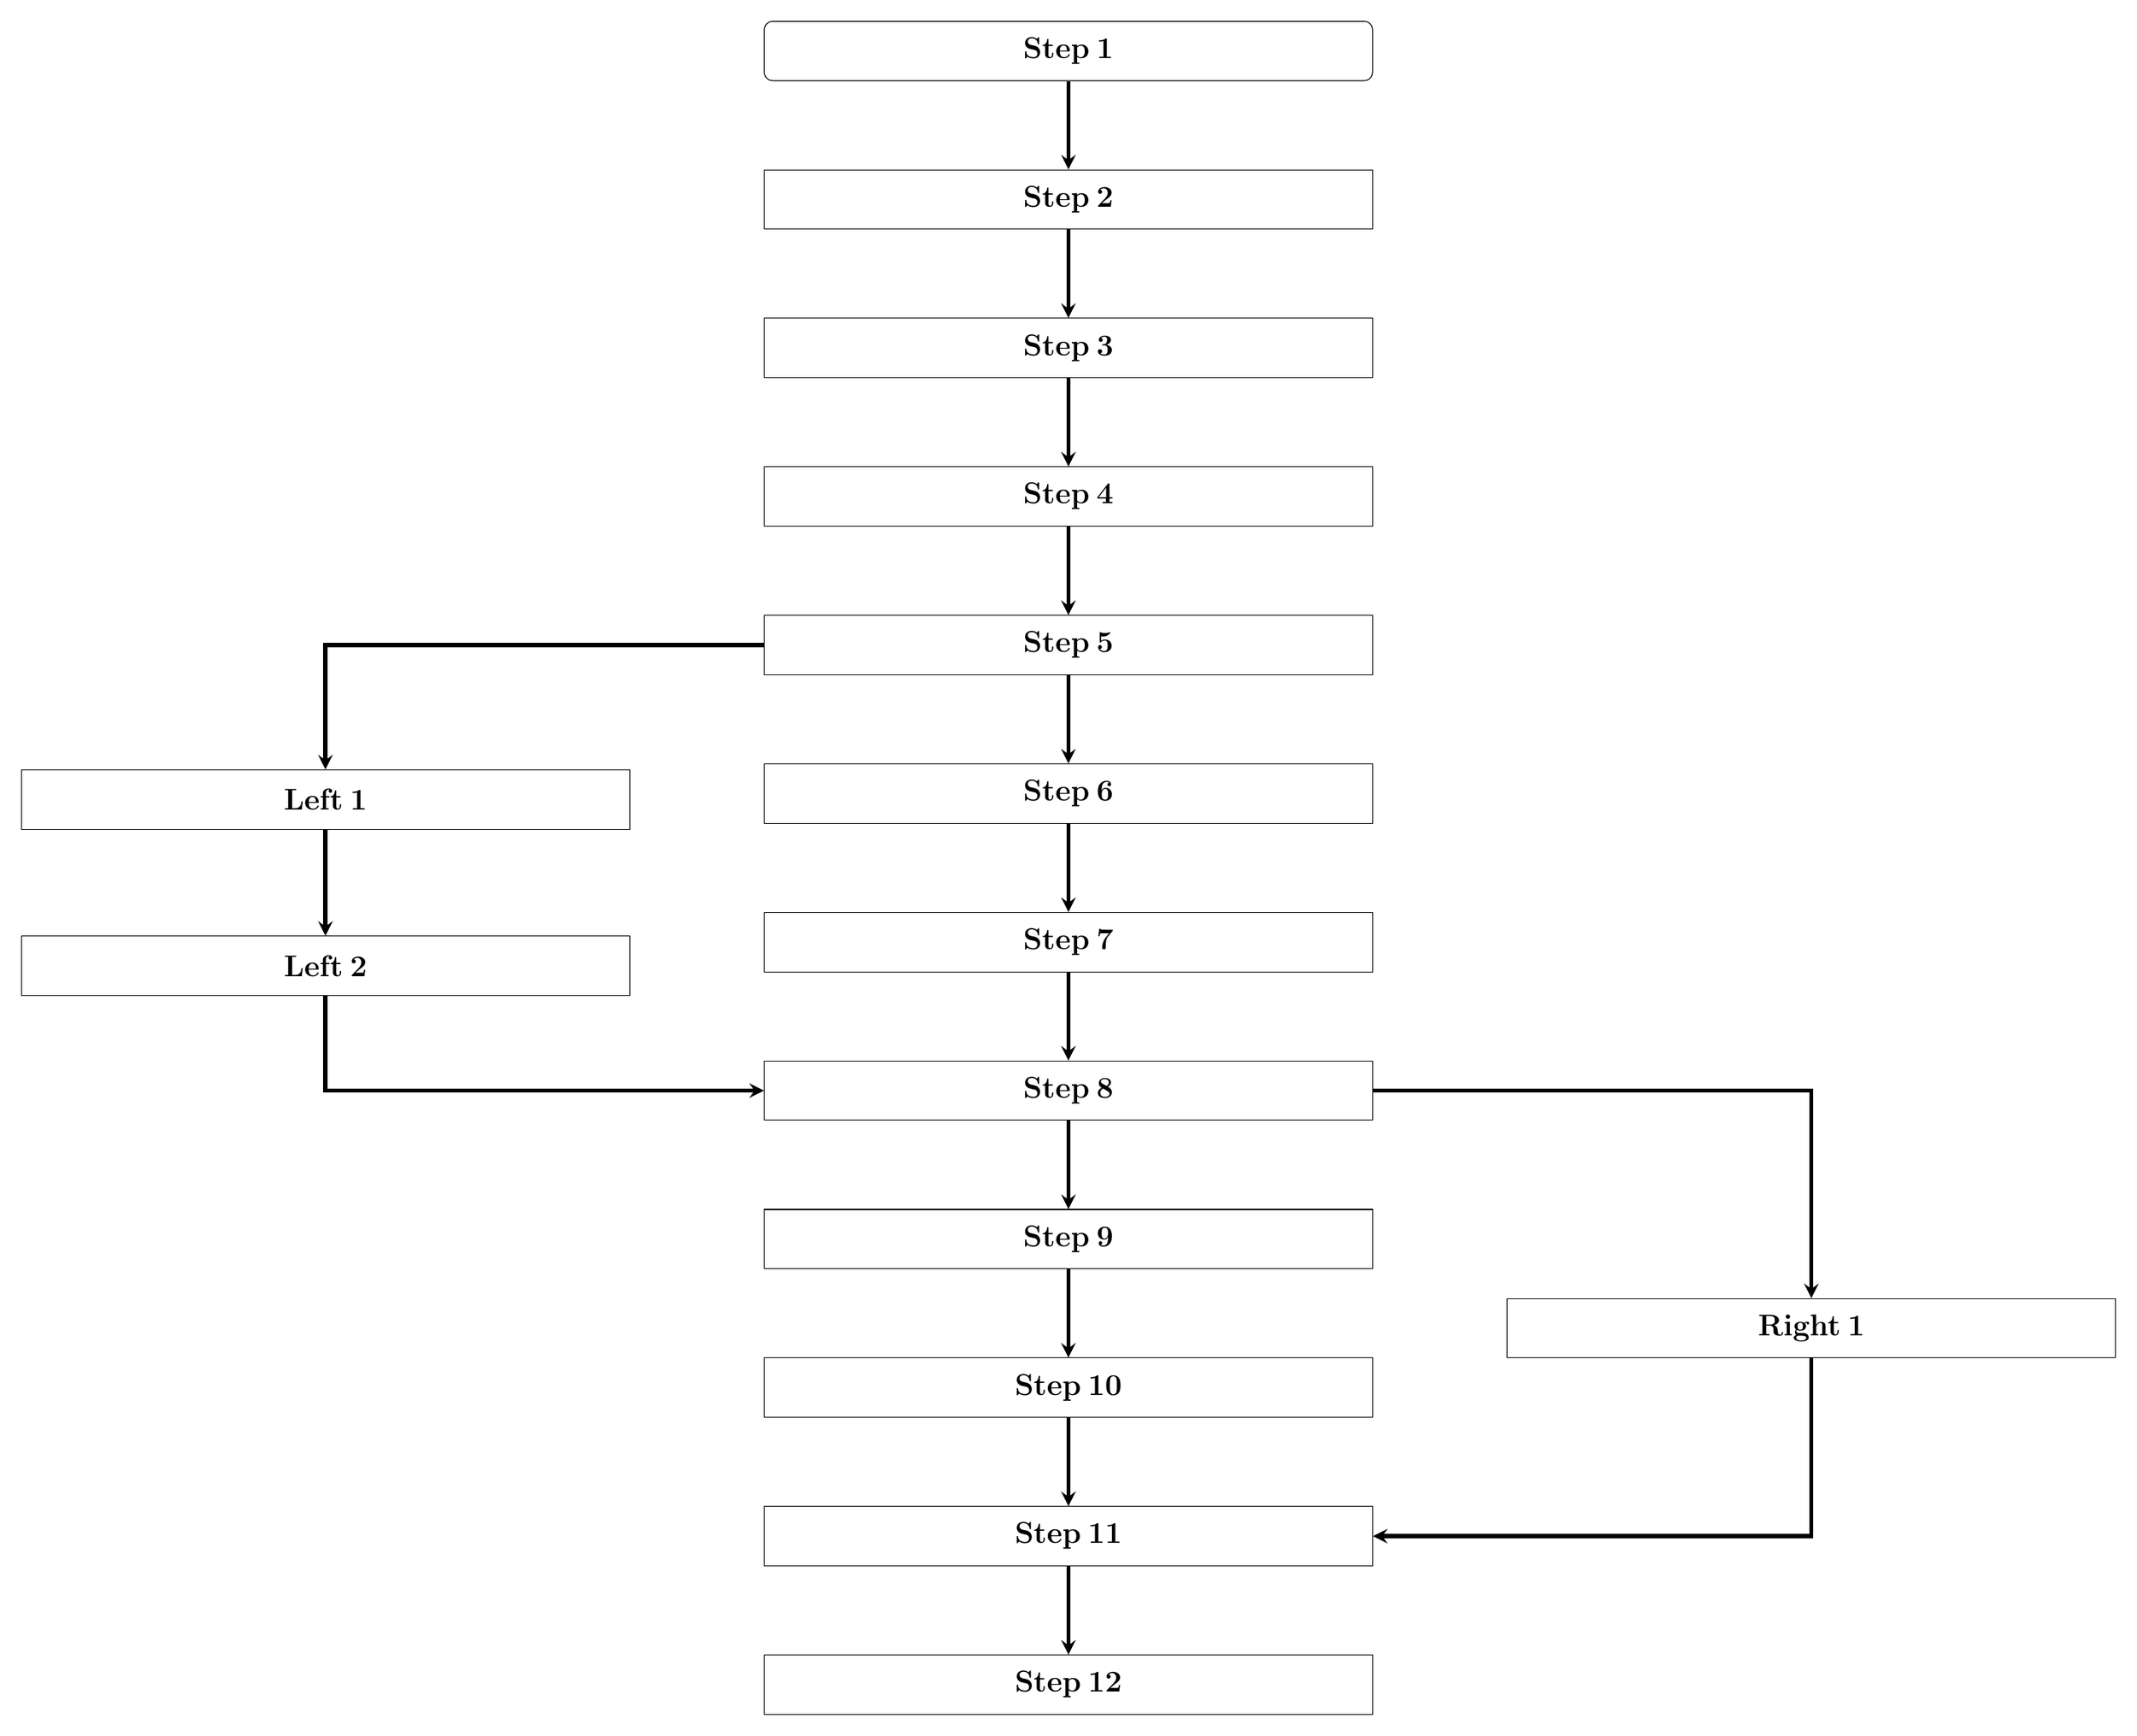
\begin{tikzpicture}[node distance=2.5cm]
                \node (t1) [startstop] {\textbf{{\Large Step 1}}};
                \node (t2) [process, below of = t1] {\textbf{{\Large Step 2}}};
                \node (t3) [process, below of = t2] {\textbf{{\Large Step 3}}};
                \node (t4) [process, below of = t3] {\textbf{{\Large Step 4}}};
                \node (t5) [process, below of = t4] {\textbf{{\Large Step 5}}};
% ---------------------------------------------
% vertical (primary) Division
% ---------------------------------------------
                % Flow

                \node (t6) [process, below of = t5] {\textbf{{\Large Step 6}}};

                \node (t7) [process, below of = t6] {\textbf{{\Large Step 7}}};

                \node (t8) [process, below of = t7] {\textbf{{\Large Step 8}}};

                \node (t9) [process, below of = t8] {\textbf{{\Large Step 9}}};

                \node (t10) [process, below of = t9] {\textbf{{\Large Step 10}}};

                \node (t11) [process, below of = t10] {\textbf{{\Large Step 11}}};

                 \node (t12) [process, below of = t11] {\textbf{{\Large Step 12}}};


% ---------------------------------------------
% All arrows (for vertical column
% ---------------------------------------------

                %  All arrows (for vertical column
                \draw [arrow] (t1) -- (t2);
                \draw [arrow] (t2) -- (t3);
                \draw [arrow] (t3) -- (t4);
                \draw [arrow] (t4) -- (t5);
                \draw [arrow] (t5) -- (t6);
                \draw [arrow] (t6) -- (t7);
                \draw [arrow] (t7) -- (t8);
                \draw [arrow] (t8) -- (t9);
                \draw [arrow] (t9) -- (t10);
                \draw [arrow] (t10) -- (t11);
                \draw [arrow] (t11) -- (t12);
% ---------------------------------------------
% Left Division
% --------------------------------------------- 
                \node (l1) [process, left of = t5, xshift=-10cm, yshift=-2.6cm] {\textbf{{\Large Left 1}}};

                \node (l2) [process, below of = l1, yshift=-0.3cm] {\textbf{{\Large Left 2}}};
                

% ---------------------------------------------
% All arrows (for the left column)
% ---------------------------------------------

                %  All arrows (for vertical column
                \draw [arrow] (t5) -| (l1);
                \draw [arrow] (l1) -- (l2);
                \draw [arrow] (l2) |- (t8);

% ---------------------------------------------
% Right Division
% ---------------------------------------------   
                \node (r1) [process, right of = t8, xshift=10cm, yshift=-4cm] {\textbf{{\Large Right 1}}};

% ---------------------------------------------
% All arrows (for right column)
% ---------------------------------------------

                %  All arrows (for vertical column
                \draw [arrow] (t8) -| (r1);
                \draw [arrow] (r1) |- (t11);
                
            \end{tikzpicture}
        \end{adjustbox}
    \end{center}
    \caption{Study methodology.}
    \label{fig:figure3_1}
\end{figure}


% \section{Models and Algorithms}
% \lipsum[1]

% Here is equation \ref{Eq3_1}.

% % Equation
% \begin{equation}
% e = \lim_{n\to\infty} \left(1+\frac{1}{n}\right)^n
% \label{Eq3_1}
% \end{equation} 

% \begin{align}
% 	x^2 -25 &= 0 \nonumber \\
% 	x^2 &= 25 \nonumber \\
% 	\therefore \Aboxed{x &= 5}
%  \label{Eq3_2}
% \end{align}



% \begin{multline}
% 	f(x) = 4xy^2 + 3x^3 - 2xy + 25x^3y^3 + 3xy - 4x^6y^6 + 3xy^2 - 2y^3\\ + a^3b^3c^4 + 3x^3 - 2xy + 25x^3y^3 + 3xy\\ - 4x^6y^6 + 3xy^2 - 2y^3 + a^3b^3c^4
% \label{Eq3_3}
% \end{multline}

% \section{Summary}
% \lipsum[2]

% Chapter Template

\chapter{Hardware Testing and Results}\doublespacing % Main chapter title

\label{Chapter4} % Change X to a consecutive number; for referencing this chapter elsewhere, use \ref{ChapterX}

\lhead{Chapter IV. \emph{Hardware Testing and Results}} % Change X to a consecutive number; this is for the header on each page - perhaps a shortened title

%----------------------------------------------------------------------------------------
%	SECTION 1
%----------------------------------------------------------------------------------------






\section{Introduction}
% \noindent
We assess and define the performance of the accelerator by incorporating it into a System-on-Chip (SoC) that utilizes the AJIT Processor. This processor issues commands to the accelerator and retrieves the data. Additionally, the entire system is linked to a Network Interface Controller (NIC), which ensures high-speed input/output for rapid image loading into memory. The system's architecture is depicted in Figure 4.1.
\begin{figure}[h]
    \centering
    % \includegraphics[width=\linewidth]{Chapters/Chapter_4/images/vcu128.jpg}
    \includegraphics[width=\linewidth]{../figures/vcu128.jpg}
    \caption{Block Diagram for SoC}
    % \label{fig:your_label}
\end{figure}
\\
The system features a 32-bit wide AJIT processor at its core. This processor uses an ACB interface to interact with memory and other modules. The AFB interface, connected to the Network Interface Controller (NIC) and the accelerator engine, is utilized to transfer configuration data from the processor and relay status flags back to it. The modules also have an ACB interface for memory access. The memory subsystem includes a DRAM controller linked to an ACB to UI conversion protocol, which translates memory requests from the ACB bus to DRAM requests and vice versa for responses. Additionally, the processor is equipped with a couple of UART interfaces for external communication. The NIC also has an interface to connect with the Xilinx MAC IP, enabling communication with the host machine via Ethernet, currently configured to operate at 100Mbps.

% This chapter provides an overview of the initial survey, which encompasses survey site selection, data collection with the help of videography, pedestrian selection, and the extraction and coding of variables from the collected data.



\subsection{Processor Code}
% \lipsum[2]
Below algorithm details the functioning of the processor code. It begins by initializing the memory spaces required by all modules, including the NIC queues, the kernel addresses for the accelerators, and the memory spaces for receiving and storing tensors during engine computation. Once the memory spaces are initialized, all NIC queues are configured and initialized, and the Network Interface Controller starts operating. The kernels are then fetched via Ethernet, followed by the input tensors . With the setup complete, the NIC is turned off, and the engine process the data stage by stage. After processing all the stages, the output data is sent to the host PC via Ethernet, where the results are verified for accuracy.
\begin{algorithm}
\caption{Pseudocode for processor}
\begin{algorithmic}[1]
    \STATE Initialize memory spaces for all modules:
    \STATE \quad \textbullet\ NIC queues
    \STATE \quad \textbullet\ Kernel addresses for accelerator
    \STATE \quad \textbullet\ Memory spaces for receiving and storing tensors
    \STATE Configure and initialize all NIC queues
    \STATE Start Network Interface Controller
    \STATE Fetch kernels via Ethernet
    \STATE while 1 do
    \STATE \quad Fetch input tensor via Ethernet
    % \STATE Turn off NIC
    \STATE \quad  Process the input
    \STATE \quad Send output data to host PC via Ethernet
    \STATE end while
\end{algorithmic}
\end{algorithm}

\section{NIC Interface}
The processor initializes the NIC queues and activates the NIC. Upon receiving data from the MAC, the NIC retrieves an address from the free queue, which contains addresses of empty packet buffers, and writes the packet to that buffer. After successfully writing the packet, the NIC places the buffer's address into the RX queue. An address in the RX queue signifies that a packet has been received and requires processor action. During this process, the processor continuously polls the RX queue. Upon detecting data, it reads the packet and makes a decision. The processor then stores the packet in a shared memory location accessible to the accelerator through its registers. Once the packet storage is complete, the processor places the address into the TX queue, serving as an acknowledgment for the host. Upon receiving this acknowledgment, the host sends a new packet. This describes the overall process for storing files in memory.\\
To transmit a file via the Ethernet interface, the processor first breaks the file into multiple packets. It then retrieves an empty buffer address from the free queue and stores each packet at the corresponding address. Once the packet is successfully stored, the processor pushes the buffer address into the TX queue. The NIC's transmit engine, which continuously polls the TX queue, reads the buffer and sends the packet out. This process is repeated until all packets are transmitted.

\section{Accelerator Interface}
% \lipsum[1]
The processor begins by loading data into registers 1 to 12. It then sets bits 0 and 2 of register 0, signaling the accelerator to commence operation. The processor can either proceed with other tasks or poll register 0, awaiting the completion signal indicated by bit 3 of register 0 being set high. Once the accelerator completes its task, the processor updates the registers with the parameters for the next stage or image.\\
Additionally, the accelerator is managed by a control daemon that resets the registers, reads data from the AFB ACCELERATOR REQUEST, writes this data to the accelerator registers, and sends back a response to the AFB ACCELERATOR RESPONSE. This control daemon runs continuously, waiting for requests from the processor on the AFB ACCELERATOR REQUEST.\\
The accelerator also includes a worker daemon that monitors the r0 register for specific bits to be set. When the processor issues an execution request through the registers, the worker daemon invokes the core function with the parameters stored by the processor in other registers. Upon completing the execution, it sets bit 3 of r0 back to 0, signaling to the processor that the computation is finished.\\


\newpage

\section{Results}
% \lipsum[1-2]
\begin{table}[h]
    \centering
    \begin{tabularx}{1.1\textwidth}{|c|X|X|c|}
        \hline
        \textbf{Sr.No} & \textbf{Platform}  & \textbf{Datatype for storage} & \textbf{Accuracy} \\
        \hline
        1 &  CPU & 32 bit float    & 98.27\% \\
        \hline
        2 &  CPU & UINT8    & 98\% \\
        \hline
        3 &  FPGA & UINT8    & 98\% \\
        \hline


    \end{tabularx}
    \caption{Comparison of LeNet Architecture on Different Platforms}
    \label{tab:lenet_comparison}
\end{table}


% \subsection{Data Extraction and Coding}
% \lipsum[13]



% \section{Summary}
% \lipsum[4]






%%%%%%%%%%%%%%%%% Changes%%%%%%%%%%%%%%%%%%%%%%%%














































 
% Chapter Template

\chapter{Summary}\doublespacing % Main chapter title

\label{Chapter5} % Change X to a consecutive number; for referencing this chapter elsewhere, use \ref{ChapterX}

\lhead{Chapter V. \emph{Summary}} % Change X to a consecutive number; this is for the header on each page - perhaps a shortened title
In this work, we present a CNN inference engine on FPGA which can produce results with higher accuracy despite storing those results in 8 bit integer format. This engine is designed using AHIR-V2 and PyAHIR tools. We demonstrate an application of the engine by developing image classification algorithm using LeNet architecture, a well known ML model for image classification.
\\
We also integrated the engine with an AJIT processor and Network Interface Controller (NIC) to generate a system-on-chip (SoC) capable of performing at-edge AI/ML inference tasks. Using the SoC, we established the correctness of the acceleration engine using a test bench to validate the output sent to the host machine after every stage.\\
Our analysis of the engine's characteristics reveals opportunities for enhancing performance and robustness. These potential optimizations are outlined as future work here:
\begin{itemize}
    \item To increase the parallel computations in the hardware, multiple copies of the engines can be deployed, where each engine will work with separate filter, but on same input. This will help in obtaining the output of multiple channels simultaneously, thus decreasing the overall inference time for the output while maintaining same hardware utilization.
    \item By supporting half precision arithmetic, a significant throughput enhancement can be achieved, stemming from the ability to perform twice the number of operations, compared to the current hardware implementation that exclusively employs single precision operators, thereby leveraging the reduced numerical precision requirements to double operational bandwidth and accelerate computational throughput. 
    \item Through hardware design optimization, the engine's hardware utilization can be maximized, facilitating the extension of its capabilities to accommodate the execution of sophisticated CNN operations, such as Batch Normalization and depthwise convolution, in addition to standard convolution operations, thereby enhancing the engine's versatility and computational range.
\end{itemize}




%----------------------------------------------------------------------------------------
%	SECTION 1
%----------------------------------------------------------------------------------------



% \section{Introduction}
% Nam dui ligula, fringilla a, euismod sodales, sollicitudin vel, wisi. Morbi auctor lorem non justo. Nam lacus libero, pretium at, 
%  obortis vitae, ultricies et, tellus. Donec aliquet.


% \section{Descriptive Statistics}
% \lipsum[2]


% \section{Model Development}
% \lipsum[2]


% \section{Discussion}
% \lipsum[1]


% \section{Summary}
% \lipsum[3]






 
% \input{Chapters/Chapter_6/Chapter6} 
% \input{Chapters/Chapter7} 





\clearpage % Start a new page
%----------------------------------------------------------------------------------------
%	THESIS CONTENT - APPENDICES
%----------------------------------------------------------------------------------------

% \addtocontents{toc}{\vspace{2em}} % Add a gap in the Contents, for aesthetics

% \appendix % Cue to tell LaTeX that the following 'chapters' are Appendices

% Include the appendices of the thesis as separate files from the Appendices folder
% Uncomment the lines as you write the Appendices

% \input{Appendices/AppendixA}
% \input{Appendices/AppendixB}
% \input{Appendices/AppendixC}
%\input{Appendices/AppendixD}

% \addtocontents{toc}{\vspace{2em}} % Add a gap in the Contents, for aesthetics

% \backmatter

%----------------------------------------------------------------------------------------
%	BIBLIOGRAPHY
%----------------------------------------------------------------------------------------

\label{References}

\lhead{\emph{References}} % Change the page header to say "Bibliography"
%\usepackage{natbib}
%\renewcommand{\refname}{References}
\renewcommand\bibname{References}
% \bibliographystyle{elsarticle-harv} % Use the "custom" BibTeX style for formatting the Bibliography
%\setcitestyle{authoryear,open={((},close={))}}

\bibliography{references} % The references (bibliography) information are stored in the file named "Bibliography.bib"
[1] Aman Dhammani, “An AI/ML Inference Engine Developed Using AHIR-V2 Tools”, [Unpublished Dual Degree Thesis, IIT Bombay]. 
\\

 [2]Mohd, Bassam \& Ahmad Yousef, Khalil \& Almajali, Anas \& Hayajneh, Thaier. (2024). Quantization-Based {Optimization} Algorithm for Hardware Implementation of Convolution Neural Networks. Electronics. 13. 1-25. 10.3390/electronics13091727. \\
 
[3] Blott, Michaela \& Preußer, Thomas \& Fraser, Nicholas \& Gambardella, Giulio \& O'Brien, Kenneth \& Umuroglu, Yaman \& Leeser, Miriam \& Vissers, Kees. (2018). FINN- R: An End-to-End Deep-Learning Framework for Fast Exploration of Quantized Neural Networks. ACM Transactions on Reconfigurable Technology and Systems. 11. 1-23. 10.1145/3242897. \\

[4] Ji, Mengfei \& Al-Ars, Zaid \& Hofstee, H.P. \& Chang, Yuchun \& Zhang, Baolin. (2023). FPQNet: Fully Pipelined and Quantized CNN for Ultra-Low Latency Image Classification on FPGAs Using OpenCAPI. Electronics. 12. 4085. 10.3390/electronics12194085. 
\\

[5] Zhang, W. A Survey of Field Programmable Gate Array-Based Convolutional Neural Network Accelerators. Int. J. Electron.Commun. Eng. 2020, 14, 419–427.\\

[6] Mittal, S. A survey of FPGA-based accelerators for convolutional neural networks. Neural Comput. Appl. 2020, 32, 1109–1139. \\

[7] Gholami, A.; Kim, S.; Dong, Z.; Yao, Z.; Mahoney, M.W.; Keutzer, K. A survey of quantization methods for efficient neuralnetwork inference. arXiv 2021, arXiv:2103.13630   \\

[8] Kim, Y.D.; Park, E.; Yoo, S.; Choi, T.; Yang, L.; Shin, D. Compression of deep convolutional neural networks for fast and lowpower mobile applications. arXiv 2015, arXiv:1511.06530. 
 \\

 [9] Qiu, J.; Wang, J.; Yao, S.; Guo, K.; Li, B.; Zhou, E.; Yu, J.; Tang, T.; Xu, N.; Song, S.; et al. Going deeper with embedded fpga platformfor convolutional neural network. In Proceedings of the 2016 ACM/SIGDA International Symposium on Field-ProgrammableGate Arrays, Monterey, CA, USA, 21–23 February 2016; pp. 26–35. 
  \\
  
  [10] Chen, T.; Du, Z.; Sun, N.; Wang, J.; Wu, C.; Chen, Y.; Temam, O. Diannao: A small-footprint high-throughput accelerator forubiquitous machine-learning. ACM SIGARCH Comput. Archit. News 2014, 42, 269–284.   \\
  
  [11] Mohd, B.J.; Hayajneh, T.; Vasilakos, A.V. A survey on lightweight block ciphers for low-resource devices: Comparative study andopen issues. J. Netw. Comput. Appl. 2015, 58, 73–93. 
    \\
    
    [12] Zhuang, B.; Shen, C.; Tan, M.; Liu, L.; Reid, I. Towards effective low-bitwidth convolutional neural networks. In Proceedings ofthe IEEE Conference on Computer Vision and Pattern Recognition, Salt Lake City, UT, USA, 18–22 June 2018; pp. 7920–7928. \\
    
[13] Zhu, C.; Han, S.; Mao, H.; Dally, W.J. Trained ternary quantization. arXiv 2016, arXiv:1612.01064 \\

[14] Miyashita, D.; Lee, E.H.; Murmann, B. Convolutional neural networks using logarithmic data representation. arXiv 2016,arXiv:1603.01025.\\
% \newpage
% % Appendix Template

\chapter{List of Publications} % Main appendix title

\label{LOP} % Change X to a consecutive letter; for referencing this appendix elsewhere, use \ref{AppendixX}

\lhead{\emph{List of Publications}} % Change X to a consecutive letter; this is for the header on each page - perhaps a shortened title

\textbf{Articles Published in International/National Journals}

\begin{enumerate}
    \item Article item 1

    \item Article item 2
\end{enumerate}

\textbf{Presentations and Proceedings in International/National Conferences}

\begin{enumerate}
    \item Conference item 1

    \item Conference item 2
\end{enumerate}
% \newpage
% % \include{Biography}


\end{document}  
